\documentclass{article}
\usepackage[utf8]{inputenc}
\usepackage{graphicx}
\usepackage[super,negative]{nth}
\usepackage{longtable}
\usepackage{multirow}
\usepackage{fancyhdr}
\usepackage{float}
\usepackage{subfig}
\usepackage{color, soulutf8}
\usepackage{graphicx}
\usepackage{grffile}

\usepackage{hyperref}
\hypersetup{
	colorlinks=true,
	linkcolor=black,
	filecolor=black,      
	urlcolor=black,
}

\usepackage[dvipsnames]{xcolor}
\usepackage{listings}

\renewcommand{\thefigure}{\arabic{section}.\arabic{figure}}
\newcommand\goal[1]{\item[{[G#1]}] }
\newcommand\requirement[1]{\item[{[R#1]}] }
\newcommand\assumption[1]{\item[{[A#1]}] }
\newcommand\usecase[1]{ [UC#1] }

\begin{document}
	\begin{titlepage}
		
		\centering
		\vspace*{0.7 cm}
		
\includegraphics[scale = 0.7]{images/PolimiLogo.png}\\[1 cm]
		\textsc{\large Dipartimento di Elettronica, Informazione e Bioingegneria}\\[2 cm]
		
		\rule{\linewidth}{0.2 mm} \\[0.5 cm]
		{\huge \bfseries Design Document (DD)}\\
		\rule{\linewidth}{0.2 mm} \\[1.5 cm]
		
		\textsc{\Large SafeStreets}\\[0.5 cm]
		\textsc{\large - v1.0 -}\\[1 cm]
		
		\begin{minipage}{\textwidth}
			\begin{flushleft} \large
				\emph{Authors:}\\
				\textbf{Quacquarelli} Sebastiano \hfill 945071 \\
				\textbf{Ricchiuti} Simone \hfill 945613  \\
				\textbf{Sala} Nicolò \hfill 945898  \\[2 cm]
			\end{flushleft}
		\end{minipage}\\[2 cm]
		
		{\large December \nth{9} , 2019}\\[2 cm]
		
	\end{titlepage}
	
	\pagenumbering{roman}
	\tableofcontents
	\clearpage
	\newpage
	\pagenumbering{arabic}
	\setcounter{page}{1}
	
	\section{Introduction}
		\subsection{Purpose}
		\subsection{Scope}
		\subsection{Definitions, Acronyms, Abbreviations}
			\subsubsection{Definitions}
			\subsubsection{Acronyms}
			\subsubsection{Abbreviations}
		\subsection{Revision history}
			\begin{table}[h]
				\centering
				\begin{tabular}{c c c}
					\hline
					\textbf{Version} & \textbf{Last update} & \textbf{Comments} \\ 
					\hline
					1.0 &  \nth{9} December, 2019  & \\
					\hline
				\end{tabular}
				\caption{Revision history}
				\label{fig:Revision history}
			\end{table}
		\subsection{Document structure}
			In this part is shown how the document has been divided. For each chapter, is given a short description:
			\begin{itemize}
				\item \textit{Chapter 1} 
				\item \textit{Chapter 2} 
				\item \textit{Chapter 3} 
				\item \textit{Chapter 4} 
				\item \textit{Chapter 5} 
				\item \textit{Chapter 6} 
				\item \textit{Chapter 7} simply includes the references.
			\end{itemize}
	\section{Architectural design}
		\subsection{Overview}
		\subsection{Component view}
		\subsection{Deployment	view}
		\subsection{Runtime	view}
		\subsection{Component interfaces}
		\subsection{Selected architectural styles and patterns}
		\subsection{Other design decision}
	\clearpage	
	\section{User Interface Design}
	To give an approximate idea of how the interfaces of the application should appear, some mockups, both for SafeStreets Application and SafeStreets AE, have been given in \href{run:d:../DeliveryFolder/RASD1.pdf}{RASD} [Section 3.1.1].\\ 
	In order to express the relations among pictures RASD [3.1.1], here it will be illustrated a pair of UX Diagrams.
	
	\begin{figure}[H]
		\centering
		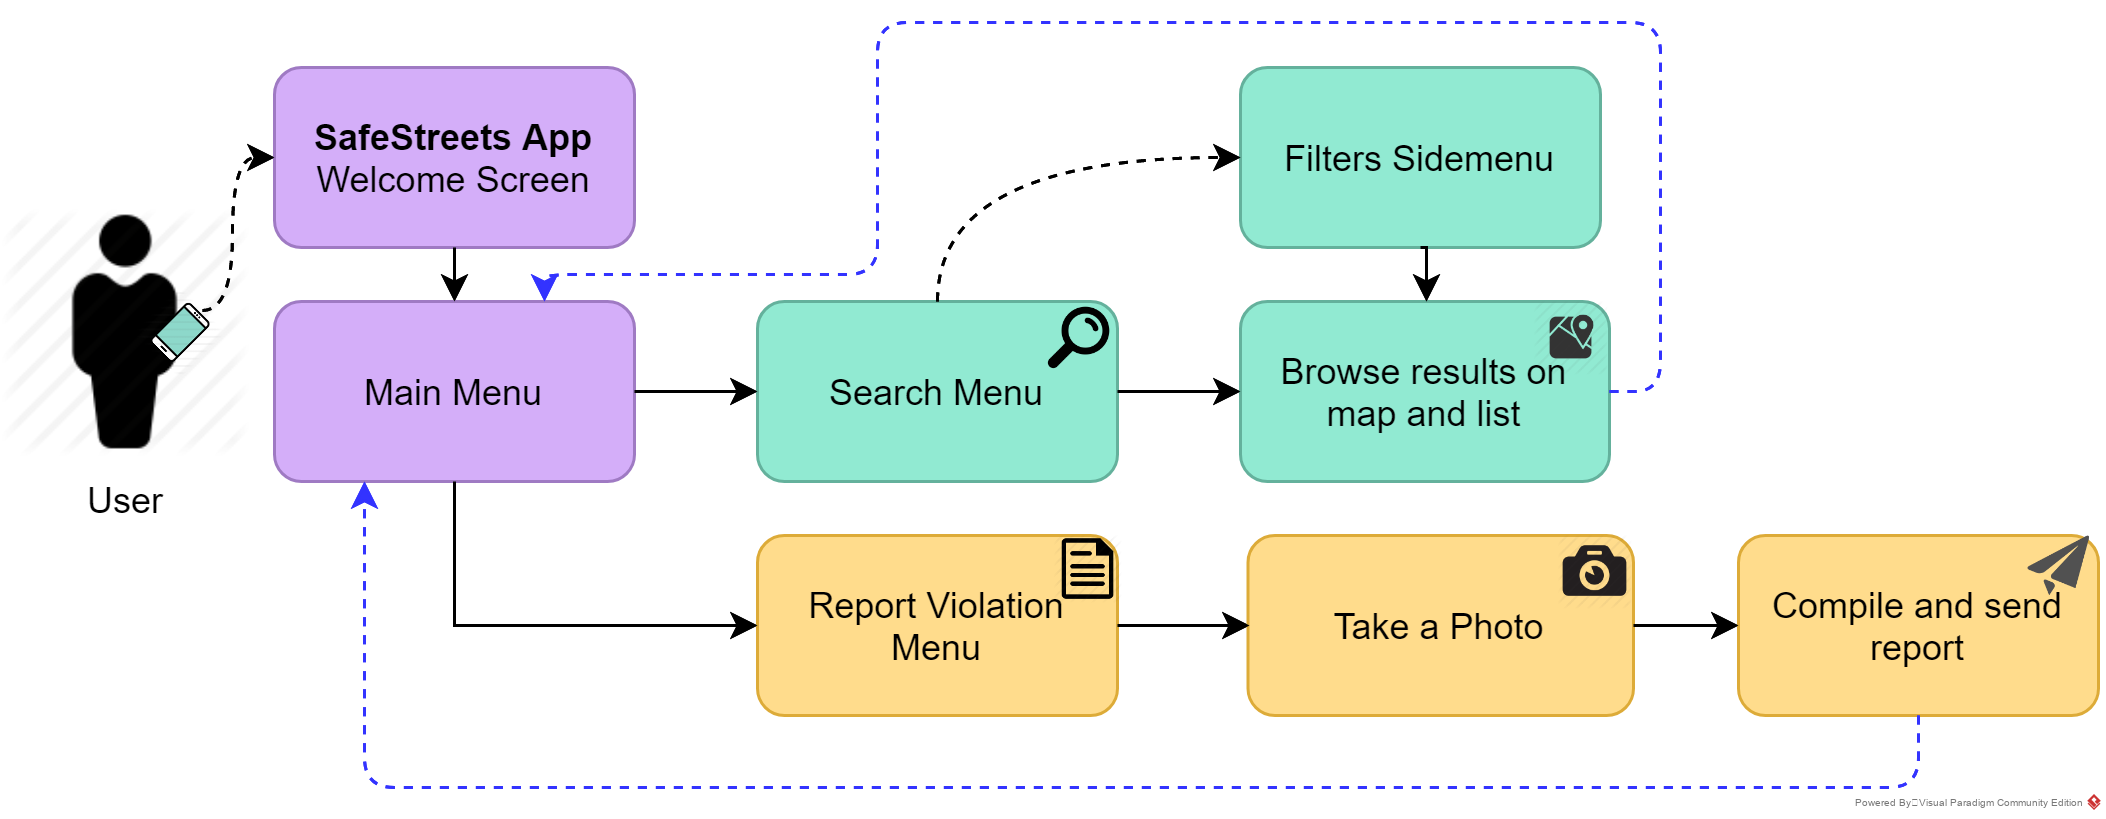
\includegraphics[width=1\textwidth]{diagrams/UXSafeStreetsApp.png}
		\caption[User Experience diagram for SafeStreets App]{User Experience diagram for SafeStreets App}
		\label{fig:UX_SSApp}
	\end{figure}

	\begin{figure}[H]
		\centering
		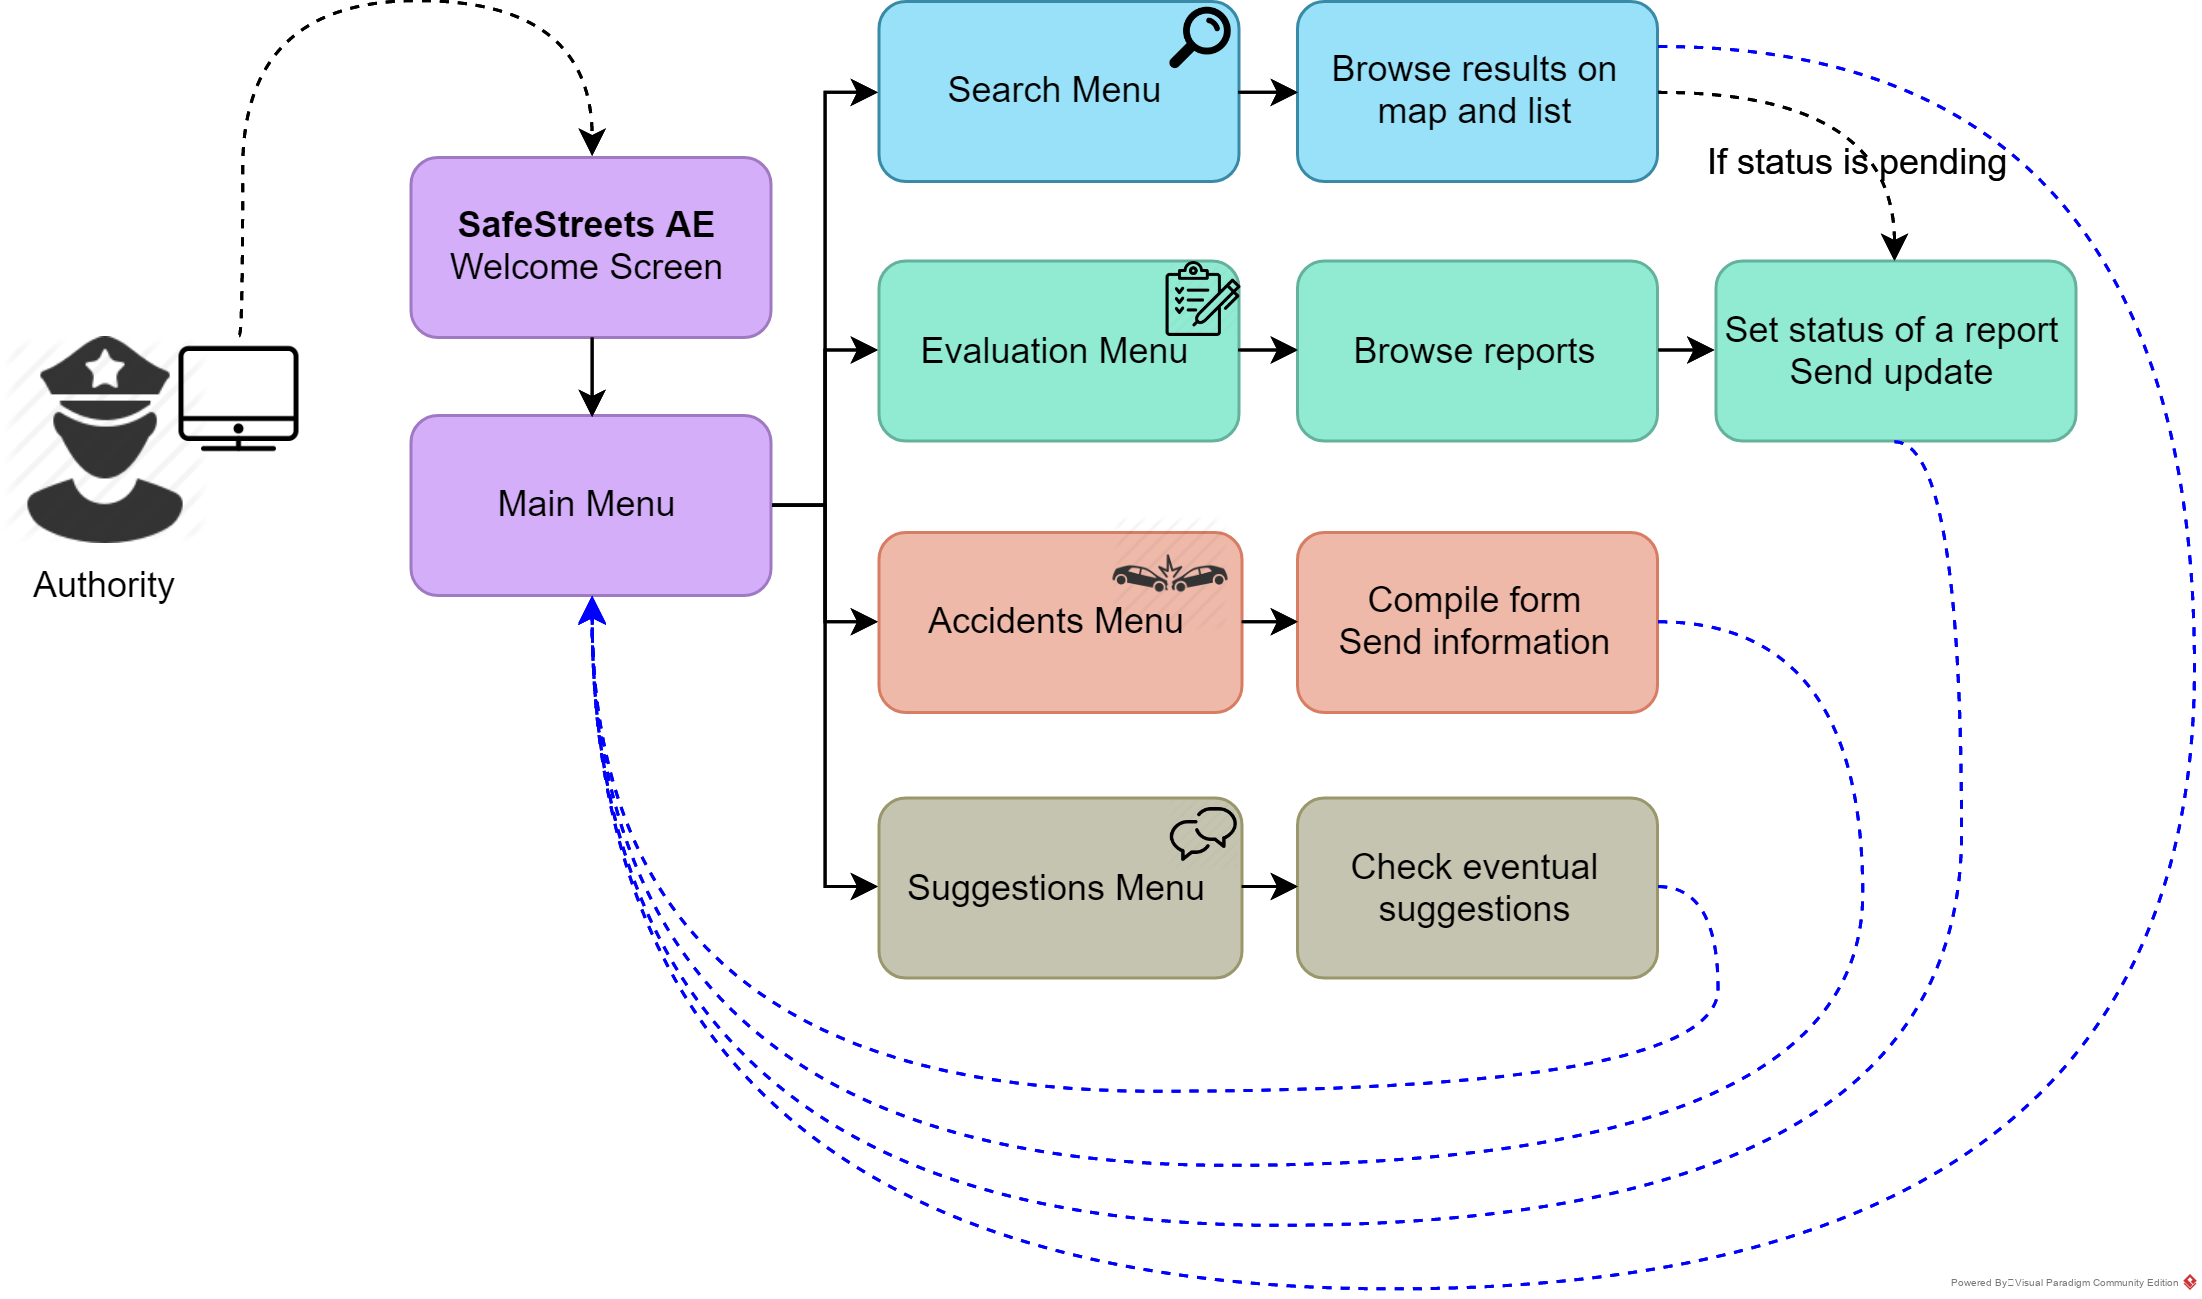
\includegraphics[width=1\textwidth]{diagrams/UXSafeStreetsAE.png}
		\caption[User Experience diagram for SafeStreets AE]{User Experience diagram for SafeStreets AE}
		\label{fig:UX_SSAE}
	\end{figure}
		
	\clearpage	
	\section{Requirements Traceability}
	\clearpage	
	\section{Implementation, integration and test plan}
	
	\clearpage
	\section{Effort Spent}
		\begin{table}[h]
			\centering
			\begin{tabular}{l c}
				\hline\hline
				\multicolumn{2}{c}{\textbf{Team Work}} \\
				\hline
				\textbf{Task} & \textbf{Hours} \\ [0.5ex]
				\hline
				Understanding the problem & 2  \\
				Brainstorming & 4 \\
				Software system attributes & 8 \\
				\hline
				\textbf{Total} & 14  \\
				\hline
			\end{tabular}
			\caption{Time spent by all team members}
			\label{fig:Time spent by all team members}
		\end{table}
		
		\begin{table}[h]
			\centering
			\begin{tabular}{l c l c l c}
				\hline\hline
				\multicolumn{6}{c}{\textbf{Individual Work}} \\
				\hline
				\multicolumn{2}{c |}{\textbf{Nicolò Sala}}  &
				\multicolumn{2}{c |}{\textbf{Sebastiano Quacquarelli}} &
				\multicolumn{2}{c}{\textbf{Simone Ricchiuti}}\\
				\hline
				\textbf{Task} & \textbf{Hours}
				& \textbf{Task} & \textbf{Hours}
				& \textbf{Task} & \textbf{Hours} \\ [0.5ex]
				\hline
				%Nicolò								Sebastiano							Simone
				Constraints & 2						& Definitions & 1					& Introduction & 4
				\\\hline
				Definitions & 1						& User interfaces. & 5				& Product functions  & 4
				\\\hline
				UC description & 3					& Domain model & 4				    & User characteristics  & 0.5 
				\\\hline
				Performance req. & 1				& UC descr./diagrams & 4			& Functional req & 2 
				\\\hline
				Design constraints & 1				& Assumptions & 2					& UC description & 3  
				\\\hline
				Alloy & 9							& Sequence diagrams & 2				& Activity Diagrams  & 2  
				\\\hline
				\textbf{Total} & 17					& \textbf{Total} & 18				& \textbf{Total} & 15.5
				\\\hline
			\end{tabular}
			\caption{Time spent by each team member}
			\label{fig:Time spent by each team member}
		\end{table}
	
	\clearpage
	\section{References}
		\begin{itemize}
			\item "2019-2020 Software Engineering 2 mandatory project: goal, schedules and rules";
			\item TeXstudio (\url{https://www.texstudio.org}) to edit the LaTeX document;
			\item Visual Paradigm CE (\url{https://www.visual-paradigm.com/}) to create UML diagrams.
		\end{itemize} 
	
\end{document}
